% Created 2013-01-04 Fr 21:21
\documentclass[11pt]{article}
\usepackage[utf8]{inputenc}
\usepackage[T1]{fontenc}
\usepackage{fixltx2e}
\usepackage{graphicx}
\usepackage{longtable}
\usepackage{float}
\usepackage{wrapfig}
\usepackage{soul}
\usepackage{textcomp}
\usepackage{marvosym}
\usepackage{wasysym}
\usepackage{latexsym}
\usepackage{amssymb}
\usepackage{hyperref}
\tolerance=1000
\providecommand{\alert}[1]{\textbf{#1}}

\title{zettelkasten}
\author{florian}
\date{\today}
\hypersetup{
  pdfkeywords={},
  pdfsubject={},
  pdfcreator={Emacs Org-mode version 7.8.11}}

\begin{document}

\maketitle

\setcounter{tocdepth}{3}
\tableofcontents
\vspace*{1cm}


\section{Zettelverwaltung}
\label{sec-1}
\subsection{\textbf{Zettel8} \textbf{Elementare Stochastik}}
\label{sec-1-1}
\subsection{\textbf{Zettel1}0 \textbf{Logik}}
\label{sec-1-2}
\subsection{\textbf{Softwaretechnik}}
\label{sec-1-3}
\subsection{\textbf{Zettel1}0 \textbf{Theoretische Informatik}}
\label{sec-1-4}
\section{Webdesign}
\label{sec-2}
\section{Elementare Stochastik}
\label{sec-3}
\subsection{Englisch}
\label{sec-3-1}


\begin{center}
\begin{tabular}{ll}
 Deutsch                    &  Englisch                        \\
\hline
 Erwartungswert             &  expected value                  \\
 exponentialverteilung      &  exponential distribution        \\
 Varianz                    &  variance                        \\
 gleichverteilung           &  uniform distribution            \\
 Irrfahrt                   &  random walk                     \\
 Wahrscheinlichkeitsdichte  &  random density                  \\
                            &  probapility density (function)  \\
 Zufallsvariable            &  random variable                 \\
\end{tabular}
\end{center}
\subsection{Verteilungen}
\label{sec-3-2}
\subsection{Bedingter Erwartungswert}
\label{sec-3-3}

A,B Ereignisse; Y Zufallvariable
$P(A|B) = \frac{P(A \cap B)}{P(B)}$ Ws A wenn B bekannt
$P(Y|B) = \frac{E(1_{B} * Y)}{P(B)}$

\texttt{Skript}
\subsection{Zusammenhänge}
\label{sec-3-4}

\begin{itemize}
\item Var(X) = Cov(X,X)
\item Cov(X,Y) = E(X*Y) - E(X)E(Y)
\end{itemize}
\subsection{Wörterbuch}
\label{sec-3-5}

\begin{description}
\item[Erwartungswert] 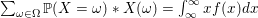
\includegraphics[width=.9\linewidth]{201301ad-2329314949s0X.png} = 
\includegraphics[width=.9\linewidth]{201301ad-23333749495-d.png}
                    für Abwandlung relativer Häufigkeit:  E(X[n])=z => E(X[n]/n)=z/n
\item[Zufallsvariable] Abbildung 
\includegraphics[width=.9\linewidth]{201212ad-1900221184eoW.png} wobei 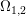
\includegraphics[width=.9\linewidth]{201212ad-1901251184ryc.png} messbare Räume
\item[messbarer Raum] existiert Abbildung Raum auf Maßraum
\item[Maßraum] der Raum in den eine Maßfunktion zuordnet (z.B. 0..1 für Ws)
\item[Wahrscheinlichkeitsfunktion] 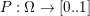
\includegraphics[width=.9\linewidth]{201212ad-190439118448i.png}
\item[Wahrscheinlichkeitsdichtefunktion] gibt zu ZVar und möglichen 
      Output die Wahrscheinlichkeit an
\item[gleichverteilt] alle outputs sind gleich wahrscheinlich
\item[Varianz] 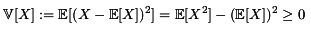
\includegraphics[width=.9\linewidth]{zettelkasten.org_20121229_215420_14976asg.png} = 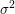
\includegraphics[width=.9\linewidth]{201212ad-21574114976n2m.png} (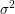
\includegraphics[width=.9\linewidth]{201301ad-00394849495FS.png} Standardabweichung)
           = irgend ein Maß für die mittleren Abweichungen vom Erwartungswert
            = 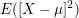
\includegraphics[width=.9\linewidth]{201301ad-0049294949gkk.png} = 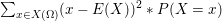
\includegraphics[width=.9\linewidth]{201301ad-0054574949tuq.png}
             Bei Binomial mit n Versuchen: 
                = n*p*(1-p)
                für Abwandlung relativer Häufigkeit: V(X[n])=z 
                   => V(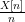
\includegraphics[width=.9\linewidth]{201301ad-1614254949GeA.png}) = 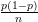
\includegraphics[width=.9\linewidth]{201301ad-1613574949UUx.png}
\item[Kovarianz] 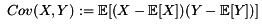
\includegraphics[width=.9\linewidth]{zettelkasten.org_20121229_220016_149760At.png} 
           = misst die zusammenhänge der Wert
               
\includegraphics[width=.9\linewidth]{conv_res.png}
            Cov(X,Y) = E(X*Y) - E(X)E(Y)
            Cov(X,Y) = Cov(Y,X)
            Cov(X+Y, Z) = Cov(X, Z) + Cov(Y, Z)
  entwicklung von X und Y, also hohe Werte von X
  => hohe Werte Y \ldots{}
\item[Tschebyscheff-Ungleichung] Mit Erwartungswert und Varianz werden Wahrscheinlichkeiten
   für Werte < Erwartungswert bestimmt/eingegrenzt (minimale Wahrscheinlichkeit)
     = 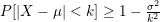
\includegraphics[width=.9\linewidth]{201212ad-07253120660_2o.png}    $\sigma$$^2$ ist varianz, $\mu$ ist Erwartungswert
\item[Wahrscheinlichkteisraum] 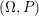
\includegraphics[width=.9\linewidth]{201212ad-15510922908saY.png} = Raum mit Ereignissen und Wahrscheinlichkeitsfunktion da drauf
\item[Indikator- / charakteristische Funktion] 1$_T$ oder \mathcal{x}_T wenn x in T 1 sonst 0
\item[Bayes - Theorem] : 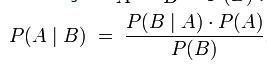
\includegraphics[width=.9\linewidth]{/home/florian/Zettelkasten/zettelkasten.org_20130103_124645_22923q8L.png}  und 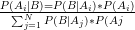
\includegraphics[width=.9\linewidth]{201301ad-12575411367wd2.png}
\end{description}
\subsection{Zettel-06}
\label{sec-3-6}
\subsubsection{Dateien}
\label{sec-3-6-1}

    \href{file:///home/florian/Dropbox/st/st-zettel-06/st-zettel-06.pdf}{st-zettel-06.pdf}
    \href{file:///home/florian/Dropbox/st/st-zettel-06/st-loesung-06.tex}{st-loesung-06.tex}
\subsubsection{Informationen}
\label{sec-3-6-2}
\begin{itemize}

\item Aufgabe 1\\
\label{sec-3-6-2-1}%
a)
$2^{-k}\binom{k}{(k+z)/2}\\$ = P(S$_k$ = w) mit w aus Omega$_n$
$2^{k}$ offensichtlich Anzahl der Blätter also auch Pfade
Damit bestimmte Nummer erreicht wird, muss es entsprechend
mehr `+1'er als `-1'er geben (k+z). (Um von k zu z zu kommen)

b) Erwartungswert ist jedenfalls 0
darauf beschränken das es gerade sein muss, zB mit 2m als index oder so

c) Wahrscheinlichkeit für Rückker bei bei unendlich ist 1
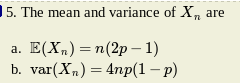
\includegraphics[width=.9\linewidth]{/home/florian/Dropbox/Zettelkasten/zettelkasten.org_20121212_065955_6717Vos.png} allgemein
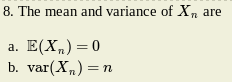
\includegraphics[width=.9\linewidth]{/home/florian/Dropbox/Zettelkasten/zettelkasten.org_20121212_070048_6717iyy.png} bei Symmetrie
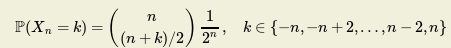
\includegraphics[width=.9\linewidth]{/home/florian/Dropbox/Zettelkasten/zettelkasten.org_20121212_070111_6717U8B.png}

$\frac{n}{2}$ einser um Zustand zu halten (rest passt dann ja),
und $\frac{k}{2}$ um da ja aufgestiegen werden soll
die müssen allen innerhalb des Pfades gezogen werden


\item Aufgabe 3\\
\label{sec-3-6-2-2}%
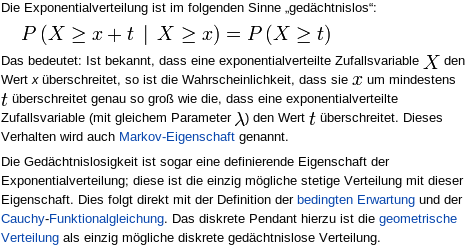
\includegraphics[width=.9\linewidth]{/home/florian/Dropbox/Zettelkasten/zettelkasten.org_20121212_071546_6717hGI.png}
==Wahrscheinlichkeit, für X >= x+t wenn X>= x schon bekannt==
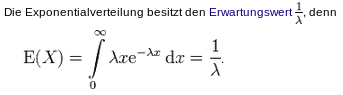
\includegraphics[width=.9\linewidth]{/home/florian/Dropbox/Zettelkasten/zettelkasten.org_20121212_084713_6717W3b.png}
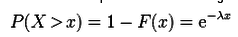
\includegraphics[width=.9\linewidth]{/home/florian/Dropbox/Zettelkasten/zettelkasten.org_20121212_082939_6717Jmh.png}

\hrule

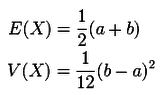
\includegraphics[width=.9\linewidth]{/home/florian/Dropbox/Zettelkasten/zettelkasten.org_20121212_095257_67179ci.png}

\end{itemize} % ends low level
\subsection{Zettel-07}
\label{sec-3-7}

\href{file:///home/florian/Dropbox/st/st-zettel-07/st-zettel-07.pdf}{st-zettel-07.pdf}
\href{file:///home/florian/Dropbox/st/st-zettel-07/st-loesung-07.tex}{st-loesung-07.tex}
\href{file://.~/Dropbox/st/st-zettel-07/st-loesung-07.pdf}{st-loesung-07.pdf }
\subsection{Zettel-08}
\label{sec-3-8}

\texttt{st-zettel-08.pdf}
\href{file:///home/florian/Dropbox/st/st-zettel-08/st-loesung-08.tex}{st-loesung-08.tex}
\subsubsection{header}
\label{sec-3-8-1}


\begin{verbatim}
\documentclass[11pt]{amsart}
\usepackage[utf8]{inputenc}
\usepackage{amssymb,amsmath}
\usepackage{verbatim}
\usepackage{color}
\usepackage{geometry}
\geometry{a4paper,left=2cm,right=2cm, top=1.5cm, bottom=1.5cm} 
\usepackage{amsthm}
\usepackage{stmaryrd}
\usepackage{graphicx}

%\includegraphics{?} setzt bild ein
%\ref{labelname} erstellt link zu labelname
%\label{labelname} kann einfach irgendwo drangesetz werden

\newtheorem{defi}{Definition}
\newtheorem{axiom}{Axiom}
\newtheorem{nota}{Notation}
\newtheorem{prop}{Proposition}
\newtheorem{satz}{Satz}
\newtheorem{umf}{Umformung}

\newenvironment{beweis}{\par\begingroup%
\settowidth{\leftskip}{\textsc{Beweis:~}}%
\noindent\llap{\textsc{Beweis:~}}}{\hfill$\Box$\par\endgroup}

\renewcommand{\baselinestretch}{1}
\newcommand{\words}{\Sigma^* \backslash \{\epsilon\}}
\newcommand{\etrans}[1]{\bar{\delta}(#1)}
\renewcommand{\P}{\mathbb{P}}

\title{Zettel 8}
\author{Florian Lerch(2404605)/Waldemar Hamm(2410010)}
%\date{} % Activate to display a given date or no date (if empty),
% otherwise the current date is printed 

\begin{document}
\maketitle
\end{verbatim}
\subsubsection{Aufgabe 1}
\label{sec-3-8-2}


\begin{verbatim}
\subsection{Aufgabe 1}
\end{verbatim}
\begin{itemize}

\item a)\\
\label{sec-3-8-2-1}%
\begin{verbatim}
\subsubsection{a)}
\end{verbatim}
Es gibt 32 Karten, 4 davon sind Buben
Jeder der 3 Spieler erhält 10 Karten
Die Wahrscheinlichkeit für einen Buben liegt bei 4/32 = 1/8 für jeden Kartenzug

\includegraphics[width=.9\linewidth]{201212ad-1238161774nwx.png} enthält die mögliche Anzahl Buben in einer Hand = \{0,1,2,3,4\}
Man kann das ganze als Binomialverteilung interpretieren, wenn die Karten mit einem mal
verteilt werden und jeder Spieler nur seine eigenen Karten kennt

\includegraphics[width=.9\linewidth]{201212ad-1302231774zON.png} die Karten somit also unabhängig voneinander sind
Als posititvis Ergebnis wird dabei das ziehen eines Buben und als negatvives Ergebnis wird das ziehen
einer anderen Karte betrachtet.
Es ergibt sich also für die Wahrscheinlichkeitsfunktion:
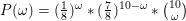
\includegraphics[width=.9\linewidth]{201301ad-17585933894AO.png}
, also alle Möglichkeiten (
\includegraphics[width=.9\linewidth]{201301ad-1800443389FLU.png}) omega mal einen Buben zu ziehen (
\includegraphics[width=.9\linewidth]{201212ad-1310561774BMy.png}) und bei allen anderen Zügen keinen (
\includegraphics[width=.9\linewidth]{201212ad-1312321774AgH.png})


\begin{verbatim}
Der Raum $\Omega$ soll die Anzahl der Buben enthalten die ein Spieler jeweils in der Hand hält. Da es nur 4
Buben gibt, gilt also: $\Omega = \{0,1,2,3,4\}$. $\mathbb{P}: \Omega \rightarrow [0,1]$ soll nun also  die Wahrscheinlichkeit
dafür darstellen, dass ein Spieler die jeweilige Anzahl Buben in seinen 10 Karten besitzt.
Bei 32 Karten und 4 Buben liegt die Wahrscheinlichkeit bei jeder einzelnen zugeteilten Karte bei $\frac{4}{32} =
\frac{1}{8}$ dafür, dass es sich um einen Buben handelt.\\
Da die Karten alle direkt zugeteilt werden und wir nur die Wahrscheinlichkeit für alle 10 Karten zusammen betrachten,
beeinflussen sich die einzelnen Karten in ihrer Wahrscheinlichkeit nicht wir können somit die Binomialverteilung
für $\mathbb{P}$ verwenden.\\
Es ergibt sich somit: $\mathbb{P}(\omega) = \binom{10}{\omega}*(\frac{1}{8})^{\omega}*(\frac{7}{8})^{10-\omega}$ für $\omega \in \Omega$
\end{verbatim}


\item b)\\
\label{sec-3-8-2-2}%
\begin{verbatim}
\subsubsection{b)}
\end{verbatim}

Aus Sicht des jeweiligen Spielers befinden sich nun noch 4 - X Karten im Spiel. Für die Karten im Skat gilt
daher das selbe Prinzip wie schon in a), d.h. Binomialverteilung.
Für beide Karten liegt die Wahrscheinlichkeit dafür, dass es sich um einen Buben handelt, bei
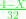
\includegraphics[width=.9\linewidth]{201212ad-1423041774NqN.png} \frac{4-X}{32} und somit kann dann der Ereignisraum 
\includegraphics[width=.9\linewidth]{201212ad-1424261774a0T.png} mit \{0,1,2\} definiert werden, und 
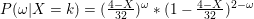
\includegraphics[width=.9\linewidth]{201301ad-1844013389GFn.png}
P($\omega$ | X = k) = (\frac{4-X}{32})$^{\omega}$ * (1 - \frac{4-X}{32})$^{\mathrm{2 - \omega}}$


\begin{verbatim}
Aus Sicht des jeweiligen Spielers befinden sich nun noch 4 - X Karten im Spiel. Für die Karten im Skat gilt
daher das selbe Prinzip wie schon in a), d.h. Binomialverteilung. \\
Sei $\Omega' = \{0,1,2\}$ und somit also die möglichen Anzahlen an Buben im Skat. \\
Analog zu a) ergibt sich für $\mathbb{P}(Y|X = k)$ nun mit für 2 Kartenziehungen und einer Wahrscheinlichkeit
von $\frac{4-X}{32}$ für einen Buben pro Karte:\\
Für $\omega \in \Omega:$ $\mathbb{P}(Y = \omega |X = k) = \binom{32}{\omega}(\frac{4-X}{32})^{\omega} * (1 - \frac{4-X}{32})^{2 - \omega}$
\end{verbatim}

\item Notizen\\
\label{sec-3-8-2-3}%
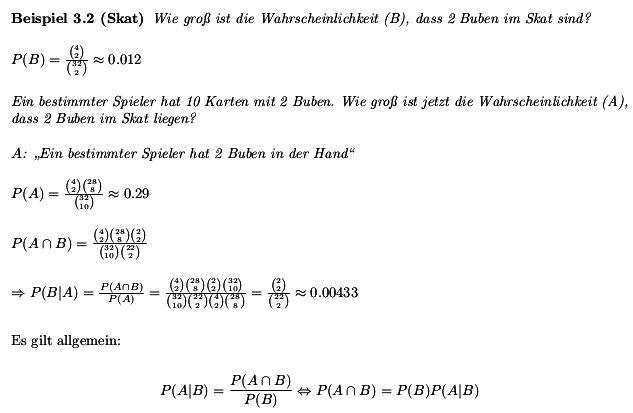
\includegraphics[width=.9\linewidth]{/home/florian/Zettelkasten/zettelkasten.org_20130103_203347_22923fmr.png}
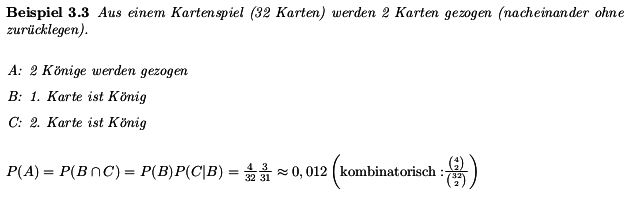
\includegraphics[width=.9\linewidth]{/home/florian/Zettelkasten/zettelkasten.org_20130103_203414_22923swx.png}
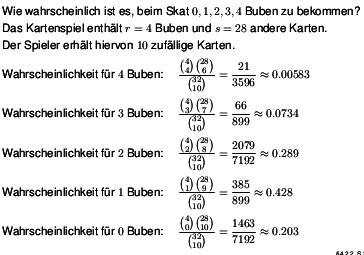
\includegraphics[width=.9\linewidth]{/home/florian/Zettelkasten/zettelkasten.org_20130103_204351_229234ON.png}
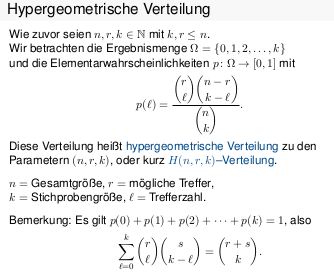
\includegraphics[width=.9\linewidth]{/home/florian/Zettelkasten/zettelkasten.org_20130103_204403_22923FZT.png}

\end{itemize} % ends low level
\subsubsection{Aufgabe 2}
\label{sec-3-8-3}


\begin{verbatim}
\subsection{Aufgabe 2}
\end{verbatim}

Fairer Würfel 2 mal geworfen
X = Augen erster Wurf
Y = Maximum beider Augenzahlen bzw. Summe
\begin{itemize}

\item a)\\
\label{sec-3-8-3-1}%
Bedingte Wahrscheinlichkeit für Y mit X = k
P(Y|X=k)
d.h. die Wahrscheinlichkeit für die Unterschiedlichen
möglichen Augen von Y, wenn k schon bekannt ist.

Durch das gegebene X verschiebt sich lediglich der Raum
der möglichen Ergebnisse für Y. Dabei wird aber keines
dieser Ergebnisse wahrscheinlicher oder Unwahrscheinlicher.

Der Bildraum ist daher: [k,12-k] $\in$ N

\begin{verbatim}
\subsubsection{a)}
Ohne Betrachtung von X gilt zunächst: $Y$ bildet auf $[2,12] \subset N$ \\
Ferner biledet X auf $[1,6] \subset N$ ab, mit gleichen Wahrscheinlichkeiten der Werte, es gilt also: $P(X=x) = \frac{1}{6}$ für $x \in [1,6]$ \\
$\Rightarrow P(Y = y | X = k) = \frac{P(X=k , Y = y)}{P(X = k)} = \frac{P(X=k , Y = y)}{6}$ \\
$ = \begin{cases} \frac{1}{6} &\mbox{falls } k < y \leq 6+k \\ 0 &\mbox{sonst} \end{cases}$ \\
\end{verbatim}

\item b)\\
\label{sec-3-8-3-2}%
g(k) = E(Y | X = k) Der Erwartungswert für ein bestimmtes Y, bei gegebenem X.
Abermals handelt es im im Grunde nur um eine simple Gleichverteilung der Wahrscheinlichkeiten in Y.
Der Erwartungswert für z.B. X wäre: E[X] = 1/6 * 1 + 1/6 * 2 \ldots{} = 1/6(1+2+3+4+5+6) = 21/6 = 3,5
Es ist anzunehmen, dass auch hier nur eine Verschiebung um k statt findet
Test X=1 Ws für Y: 1/6(2+3+4+5+6+7) = 27/6 = 9/2 = 4,5  \textbf{passt}
Test X=2 Ws für Y: 1/6(3+4+5+6+7+8) = 33/6 = 11/2 = 5,5 \textbf{passt}

\begin{verbatim}
\subsubsection{b)}
$g(k) := E[Y|X=k] = \sum_yy*P(Y=y | X = k) = \sum_{k < y \leq k+6}y*\frac{1}{6} = \frac{1}{6} * (k+1 + ... + k+6) = \frac{21}{6}*k = 3,5k$
\end{verbatim}


\item c)\\
\label{sec-3-8-3-3}%
E[Y] und E[g(X)]

Für E[Y] ist die Summe des ersten Wurfes unbekannt. Aus diesem Grund, sind die einzelnen Ergebnisse nichmehr
nur um eine Konstante verschoben und sind auch nicht mehr alle gleich wahrscheinlich.
Die Ws Verteilung wird zur Mitte hin spitzer und sollte Symmetrisch sein, so dass 5,5 der Erwartungswert sein sollte.
Stimmt nicht, die Symmetrie ist so gar nicht gegeben, da die 0 fehlt. Daher ist auch E[X] = 3,5 und nicht 3.
Neuer Tipp: 7  Kann man Erwartungswerte vielleicht addieren? Eigentlich spricht nichts dagegen. E[X] = E[Z] = 3,5
Y als die Summe aus beidem ist daher 7.

E[g(X)] = Erwartungswert des Erwartungswertes? o.O

Was ist g(X)? g(k) := E(Y | X = k)
g(X) = E(Y | X = X) oO
= E(Y) ? das ist ja schon das andere

E[ 3,5 + k] <= würde nicht gehen bzw. wäre konstant da k konstant aber:
E[3,5 + X] = 3,5 + E[X]  <= wäre nicht unbedingt so machbar. 

\textbf{E[g(X)] = E[E(Y|X)]}   <=== wichtig, fest definiert


\begin{verbatim}
\subsubsection{c)}
Sei Z die Augenzahl des 2. Wurfes, so das gilt Y = X+Z \\
$\Rightarrow E[Y] = E[X+Z] = E[X]+E[Z] = 3,5 + 3,5 = 7$ \\
$E[g(X)] = E[E(Y|X)] = E[\sum_yy*P(Y=y | X )] = \sum_x[\sum_yy*P(Y=y|X=x)]*P(X=x)$ \\
$= \sum_x\sum_yy*P(Y=y|X=x)*P(X=x) = \sum_yy*\sum_xP(Y=y, X=x) = \sum_yy*P(Y=y) = E(Y) = 7$ \\
\end{verbatim}
   
\end{itemize} % ends low level
\subsubsection{Aufgabe 3}
\label{sec-3-8-4}


\begin{verbatim}
\subsection{Aufgabe 3}
\end{verbatim}
\begin{itemize}

\item a)\\
\label{sec-3-8-4-1}%
\begin{verbatim}
\subsubsection{a)}
\end{verbatim}

\begin{itemize}
\item X, Y Zufallsvariablen -> aus ereignisraum in anderen raum
\item 
\includegraphics[width=.9\linewidth]{201212ad-1854041184ReQ.png} => existiert also
\item X$^2$ <=> Quadrat der jeweiligen Outputs
\item 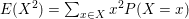
\includegraphics[width=.9\linewidth]{201212ad-21415714976zNO.png}
 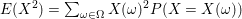
\includegraphics[width=.9\linewidth]{201212ad-21480714976AYU.png}
\end{itemize}
E(X$^2$) = $\sum$$_{\omega \in \Omega}$X($\omega$)$^{\mathrm{2P}}$(X=X($\omega$))

 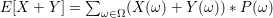
\includegraphics[width=.9\linewidth]{201212ad-05550220660LHc.png}
E[X+Y] = $\sum$$_{\omega \in \Omega}$(X($\omega$)+Y($\omega$))*P($\omega$)

Bekannt:
 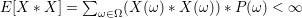
\includegraphics[width=.9\linewidth]{201212ad-05585120660YRi.png}
E[X*X] = $\sum$$_{\omega \in \Omega}$(X($\omega$)*X($\omega$))*P($\omega$) < $\infty$


=> Cov(X+Y, X-Y) = E[ (X+Y) * (X-Y) ] - E(X+Y)E(X-Y)
                    = E[ X$^2$ - Y$^2$ ] - E(X+Y)E(X-Y)

                 = E[ ([X+Y]-E[X+Y]) * ([X-Y] - E[X-Y])  ]
                    = E[  [X+Y][X-Y] - [X+Y]E[X-Y] - E[X+Y][X-Y] + E[X+Y]E[X-Y]   ]
       = E[  X$^2$ - Y$^2$ - (E[X-Y]X + E[X-Y]Y) - (E[X+Y]X - E[X+Y]Y) + E[X+Y]E[X-Y]  ]
       = E[  X$^2$ - Y$^2$ - E[X-Y]X - E[X-Y]Y - E[X+Y]X + E[X+Y]Y + E[X+Y]E[X-Y]  ]

=> Cov(X+Y, X-Y) = Cov(X,X-Y) + Cov(Y,X-Y) = Cov(X-Y,X) + Cov(X-Y, Y) = Cov(X,X) - Cov(Y,X) + Cov(X,Y) - Cov(Y,Y) = Cov(X,X) - Cov(Y,Y)
= Var(X) - Var(Y) = 0 (da gleichverteilt)

\begin{verbatim}
Da X und Y gleichverteilt sind, gilt: $Var(X) = Var(Y) \rightarrow Var(X) - Var(Y) = 0$\\
Durch die symmetrie der Kovarianz lässt sich umformen:\\
$Cov(X+Y, X-Y) = Cov(X,X-Y) + Cov(Y,X-Y) = Cov(X-Y,X) + Cov(X-Y, Y) = Cov(X,X) - Cov(Y,X) + Cov(X,Y) - Cov(Y,Y)$\\
$ = Cov(X,X) - Cov(Y,Y) = Var(X) - Var(Y) = 0$
\end{verbatim}


\item b)\\
\label{sec-3-8-4-2}%
\begin{verbatim}
\subsubsection{b)}
\end{verbatim}


\begin{verbatim}
Für Unabhängigkeit müsste gelten: $\mathbb{P}([X+Y]*[X-Y]) = \mathbb{P}(X+Y)*\mathbb{P}(X-Y) \Leftrightarrow \mathbb{P}(X^2 - Y^2) = \mathbb{P}(X+Y)*\mathbb{P}(X-Y)$ \\
Es gelte $\mathbb{P}(z) = \begin{cases} 1 &\mbox{falls } z=-1 \\ 0 &\mbox{sonst} \end{cases}$
\begin{tabbing}
Sei X = 0 und Y = 1 \=$\Rightarrow \mathbb{P}(X^2-Y^2) = \mathbb{P}(-1) = 1$ \\
\> $\Rightarrow \mathbb{P}(X+Y)*\mathbb{P}(X-Y) = \mathbb{P}(1)*\mathbb{P}(-1) = 0*1 = 0 \not = 1$ 
\end{tabbing}
$\Rightarrow$ in diesem Beispiel sind die Zufallsvariablen X+Y und X-Y zwar unkorelliert (Kovarianz ist 0) aber nicht unabhängig.
\end{verbatim}


\item Lösung Wikipedia:\\
\label{sec-3-8-4-3}%
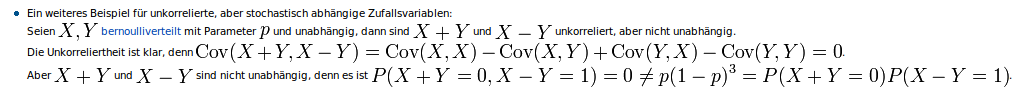
\includegraphics[width=.9\linewidth]{/home/florian/Zettelkasten/zettelkasten.org_20121230_061645_20660lbo.png}

\end{itemize} % ends low level
\subsubsection{Aufgabe 4}
\label{sec-3-8-5}


\begin{verbatim}
\subsection{Aufgabe 4}
\end{verbatim}
\begin{itemize}

\item a)\\
\label{sec-3-8-5-1}%
\begin{verbatim}
\subsubsection{a)}
\end{verbatim}

n = Anzahl Würfel
S$_n$ = Anzahl Erfolge (1 gewürfelt)
Ws für Erfolg = 1/5
Würfel haben kein Gedächtnis -> binomialverteilung
mit 1/5 erfolg und 4/5 misserfolg

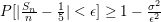
\includegraphics[width=.9\linewidth]{201212ad-07284220660MBv.png}
P[|\frac{S_n}{n} - \frac{1}{5}| < $\epsilon$] \geq 1 - \frac{\sigma^2}{\epsilon^2} 

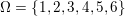
\includegraphics[width=.9\linewidth]{201212ad-07460520660LVE.png}
$\Omega$ = \{1, 2, 3, 4, 5, 6\}
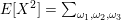
\includegraphics[width=.9\linewidth]{201212ad-07463620660lpQ.png}
E[X$^2$] = $\sum$$_{\omega_1, \omega_2, \omega_3}$

S$_n$ = Anzahl der einser bei den Würfen, und n = Anzahl der Würfel
=> 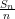
\includegraphics[width=.9\linewidth]{201301ad-2323424949SgL.png} sollte 
\includegraphics[width=.9\linewidth]{201301ad-2323574949fqR.png} ergeben, bzw. dorthin streben
\includegraphics[width=.9\linewidth]{201301ad-2334504949GJk.png}

\includegraphics[width=.9\linewidth]{201301ad-005922494964w.png} 

V(X) = E([X - E(X)]^2) = E([X-\frac{1}{5}]^2) = E(X$^2$ - 2 \frac{X}{5} + \frac{1}{25})

Var(X) = 1/5 * 4/5 * n = 4n/25



\includegraphics[width=.9\linewidth]{201301ad-0047544949Tae.png}

P[|\frac{S_n}{n} - \frac{1}{5}| < $\epsilon$] \geq 1 - \frac{4n}{25 * \epsilon^2}


\begin{verbatim}
Die Wahrscheinlichkeit für einen erfolgreichen Wurf (eine 1) liegt bei $\frac{1}{5}$ und für einen 
nicht erfolgreichen Wurf (ungleich 1) somit bei $1 - \frac{1}{5} = \frac{4}{5}$ \\
Da die einzelnen Würfe keinen Einfluss aufeinander nehmen und jeder Wurf klar in Erfolg und Misserfolg 
getrennt werden kann, lässt sich die Varianz der Normalverteilung verwenden, und es ergibt sich: \\
$Var(S_n) = n * \frac{1}{5} * \frac{4}{5} =  \frac{4n}{25}$ \\
$\Rightarrow Var(\frac{S_n}{n}) = \frac{4}{25n}$ \\
Für den Erwartungswert gilt aufgrund der Binomialverteilung: $E(S_n) = \frac{n}{5}$ \\
$\Rightarrow E(\frac{S_n}{n}) = \frac{1}{5}$ \\
Eingesetzt in die Ungleichung ergibt sich somit: $P[|\frac{S_n}{n} - \frac{1}{5}| < \epsilon] \geq 1 - \frac{4}{25n * \epsilon^2}$
\end{verbatim}

\begin{itemize}

\item Analoge Lösung mit Münze(a)\\
\label{sec-3-8-5-1-1}%
Münze positiv oder negativ, analog zu den möglichen Ergebnissen 
des Würfels (1 oder nicht 1)
\includegraphics[width=.9\linewidth]{/home/florian/Zettelkasten/zettelkasten.org_20121230_074751_20660yzW.png}

\end{itemize} % ends low level

\item b)\\
\label{sec-3-8-5-2}%
\begin{verbatim}
\subsubsection{b)}
\end{verbatim}

e = 0,001
Wie viele Würfe n nötig, damit Ws > 0.95

Eingesetzt:

ges: 1 - \frac{4}{25n * 0.001^2} > 0.95
<=> 1 - \frac{4}{0.000025n} > 0.95
=> 1 - 0.95 > \frac{4}{0.000025n}
=> 0.05 > \frac{4}{0.000025n} => 0.05 > \frac{4000000}{25n}
=> 0.05 > \frac{1}{160000n}

0.05 = \frac{1}{160000n}
0.05 = \frac{1}{n} * \frac{1}{160000} 
=> 80000 = \frac{1}{n}
=> n = \frac{1}{80000}
 

\begin{verbatim}
Es soll gelten: $1 - \frac{4}{25n * 0.000001} > 0.95$ \\
$\Leftrightarrow 1-0.95 > \frac{4}{25n * 0.000001}$ \\
$\Leftrightarrow 0.05 > \frac{160000}{n}$ \\
$\Leftrightarrow n > 3 200 000$
\end{verbatim}

\end{itemize} % ends low level
\subsubsection{Aufgabe 5}
\label{sec-3-8-6}


\begin{verbatim}
\subsection{Aufgabe 5}
\end{verbatim}
\begin{itemize}

\item a)\\
\label{sec-3-8-6-1}%
\begin{verbatim}
\subsubsection{a)}
\end{verbatim}

Berechnen Sie: \includegraphics[width=.9\linewidth]{201301ad-12403211367WJq.png}

\begin{description}
\item[1] Wo steht das Auto
\item[2] Welche Tür wählt der Kandidat
\item[3] Welche Tür öffnet der Showmaster daraufhin
\end{description}

Insgesamt existieren 3 * 3 * 3 = 27 Mögliche Kombinationien
Sei j = 1 (für jede andere Zahl gleich):
    (1,1,2) , (1,1,3) , (1,2,3), (1,3,2) => |G$_j$| = 4 Möglichkeiten, bei 2 Erfolg => 1/2 für erfolg gleich bleiben
Sei k = 1: 
    (1,1,2) , (1,1,3) , (2,1,3) , (3,1,2) => |W$_k$| = 4 , bei 2 Erfolg

\begin{center}
\begin{tabular}{ll}
 W$_k$  &  = 4  \\
\end{tabular}
\end{center}


Sei l = 1: 
    (2,2,1) , (2,3,1), (3,2,1) , (3,3,1) => |M$_l$| = 4, bei 2 Erfolg

Mit einer Wahrscheinlichkeit von 2/4 konnte der Moderator frei entscheiden, welche Tür er wählt => tür richtig
Mit einer Wahrscheinlichkeit von 2/4 musste er eine bestimmte Tür nehmen => tür falsch

Fall 1: auto getroffen => es existieren 2 andere Möglichkeiten für den Moderator, eine Tür zu wählen
Fall 2: auto nicht getroffen => es existiert nur eine andere Möglichkeit für den Moderötor, eine Tür zu wählen
=> Ws 2/3 das man das Auto vor der Wahl des Moderators nicht getroffen hatte


\includegraphics[width=.9\linewidth]{201301ad-19123649498Bz.png}


\includegraphics[width=.9\linewidth]{/home/florian/Zettelkasten/zettelkasten.org_20130103_153119_2292345w.png}

\includegraphics[width=.9\linewidth]{/home/florian/Zettelkasten/zettelkasten.org_20130103_153351_22923qDA.png}

\includegraphics[width=.9\linewidth]{/home/florian/Zettelkasten/zettelkasten.org_20130103_153423_229233NG.png}

\includegraphics[width=.9\linewidth]{/home/florian/Zettelkasten/zettelkasten.org_20130103_153540_22923EYM.png}

\includegraphics[width=.9\linewidth]{/home/florian/Zettelkasten/zettelkasten.org_20130103_153611_22923RiS.png}

\includegraphics[width=.9\linewidth]{/home/florian/Zettelkasten/zettelkasten.org_20130103_162431_22923r9S.png}

\includegraphics[width=.9\linewidth]{/home/florian/Zettelkasten/zettelkasten.org_20130103_162552_229234HZ.png}

P(A$_i$|B) = \frac{P(A_i) * P(B | A_i)}{P(A_1) * P(B | A_1) + P(A_2) * P(B | A_2) + P(A_3) * P(B | A_3)}


Gesucht: \includegraphics[width=.9\linewidth]{201301ad-1914034949uLC.png}  => Ws dass hinter j das Auto steckt, wenn wir k gewählt haben, und der Moderator Tür l geöffnet hat



Anwendung Bayes
= \frac{\frac{1}{3} * P( W_k \cap M_l | G_j)}{...}

Für festes j bleiben noch 9 (= 3*3) mögliche Elemente aus Omega,

Der Moderator darf nur Türen wählen, die nicht ungleich j sind bleiben noch 6 (= 3*2) Zustände
(1,1,2),(1,1,3),(1,2,2),(1,2,3),(1,3,2),(1,3,3)
Da darüber hinaus der Moderator aber auch nur Türen wählen kann, die ungleich k sind, bleiben noch 4 (= 2*2) Zustände
(1,1,2),(1,1,3),(1,2,3),(1,3,2)

Folglich ist P( W$_k$ $\cap$ M$_l$ | G$_j$) = \frac{4}{9}


\begin{verbatim}
$G_j = \{ (j,\omega_2,\omega_3) | \omega_2 \in \{ 1,2,3 \}, \omega_3 \in \{ 1,2,3 \} \backslash  \{ j , \omega_2 \} \}$ \\
        $= \{ \omega \in \Omega | \omega_1 = j \wedge \omega_3 \not = j \wedge \omega_3 \not = \omega_2\ \wedge \omega_3 \not = j \}$ \\
$W_k = \{ ( \omega_1 , k , \omega_3 ) | \omega_1 \in \{ 1,2,3 \} , \omega_3 \in \{ 1, 2, 3 \} \backslash \{\omega_1 , k \} \}$ \\
     $= \{ \omega \in \Omega | \omega_2 = k \wedge \omega_3 \not = k \wedge \omega_3 \not = \omega_1 \wedge \omega_3 \not = k \}$ \\
$M_l = \{ ( \omega_1 , \omega_2 , l ) | \omega_1 \in \{ 1,2,3 \} \backslash \{ l \} , \omega_2 \in \{ 1, 2, 3 \}  \backslash \{ l \} , l \}$ \\
     $= \{ \omega \in \Omega | \omega_1 \not = l \wedge \omega_2 \not = l \wedge \omega_3 = l \}$ \\

$W_k \cap M_l = \{ (\omega \in \Omega | \omega_1 \not = l , \omega_2 = k \not = l, \omega_3 = l \}$ \\

$P(G_j | W_k \cap M_l , 1 \leq j,k,l \leq 3 ) = \frac{P(W_k \cap M_l) * P(G_j)}{P(W_k \cap M_l)}$ \\

p(W_k \cap M_l | G_j ) = \begin{cases} \frac{ &\mbox{falls } k=j \\ 0 &\mbox{sonst} \end{cases}

= $\frac{P(W_k \cap M_l | G_j ) * \frac{1}{3}} {P(W_k \cap M_l)}$    

P(G_j) = 1/3
P(

bla
\end{verbatim}



\item b)\\
\label{sec-3-8-6-2}%
\begin{verbatim}
\subsubsection{b)}
\end{verbatim}


\begin{verbatim}

\end{verbatim}
\begin{itemize}

\item Bäume\\
\label{sec-3-8-6-2-1}%
\includegraphics[width=.9\linewidth]{/home/florian/Zettelkasten/zettelkasten.org_20130103_152052_22923ERY.png}
\includegraphics[width=.9\linewidth]{/home/florian/Zettelkasten/zettelkasten.org_20130103_152307_22923elk.png}
\includegraphics[width=.9\linewidth]{/home/florian/Zettelkasten/zettelkasten.org_20130103_162727_22923FSf.png}

\includegraphics[width=.9\linewidth]{/home/florian/Zettelkasten/zettelkasten.org_20130103_203554_22923e6A.png}
\includegraphics[width=.9\linewidth]{/home/florian/Zettelkasten/zettelkasten.org_20130103_203606_22923rEH.png}
\end{itemize} % ends low level

\item c)\\
\label{sec-3-8-6-3}%
\begin{verbatim}
\subsubsection{c)}
\end{verbatim}


\begin{verbatim}

\end{verbatim}
\end{itemize} % ends low level
\subsubsection{Aufgabe 6}
\label{sec-3-8-7}
\begin{itemize}

\item Cancer Rate\\
\label{sec-3-8-7-1}%
\includegraphics[width=.9\linewidth]{/home/florian/Zettelkasten/zettelkasten.org_20130103_161650_22923esY.png}
\includegraphics[width=.9\linewidth]{/home/florian/Zettelkasten/zettelkasten.org_20130103_161706_22923r2e.png}
\includegraphics[width=.9\linewidth]{/home/florian/Zettelkasten/zettelkasten.org_20130103_161729_229234Al.png}


\item nochmal mit Aids\\
\label{sec-3-8-7-2}%
\includegraphics[width=.9\linewidth]{/home/florian/Zettelkasten/zettelkasten.org_20130103_162118_22923SVx.png}
\includegraphics[width=.9\linewidth]{/home/florian/Zettelkasten/zettelkasten.org_20130103_162138_22923EfA.png}
\includegraphics[width=.9\linewidth]{/home/florian/Zettelkasten/zettelkasten.org_20130103_162207_22923RpG.png}

\item Sterbetafeln\\
\label{sec-3-8-7-3}%
\includegraphics[width=.9\linewidth]{/home/florian/Zettelkasten/zettelkasten.org_20130103_163636_22923Scl.png}
\end{itemize} % ends low level
\subsubsection{footer}
\label{sec-3-8-8}


\begin{verbatim}
\end{document}
\end{verbatim}
\subsection{Zettel-09}
\label{sec-3-9}

\href{file://.~/Dropbox/st/st-zettel-09/st-zettel-09.pdf}{st-zettel-09.pdf}
\href{file://.~/Dropbox/st/st-zettel-09/st-loesung-09.tex}{st-loesung-09.tex}
\href{file://.~/Dropbox/st/st-zettel-09/st-loesung-09.pdf}{st-loesung-09.pdf}
\subsection{Zettel-10}
\label{sec-3-10}

\href{file://.~/Dropbox/st/st-zettel-10/st-zettel-10.pdf}{st-zettel-10.pdf}
\href{file://.~/Dropbox/st/st-zettel-10/st-loesung-10.tex}{st-loesung-10.tex}
\href{file://.~/Dropbox/st/st-zettel-10/st-loesung-10.pdf}{st-loesung-10.pdf}
\subsection{Zettel-11}
\label{sec-3-11}

\href{file://.~/Dropbox/st/st-zettel-11/st-zettel-11.pdf}{st-zettel-11.pdf}
\href{file://.~/Dropbox/st/st-zettel-11/st-loesung-11.tex}{st-loesung-11.tex}
\href{file://.~/Dropbox/st/st-zettel-11/st-loesung-11.pdf}{st-loesung-11.pdf}
\section{Theoretische Informatik}
\label{sec-4}
\subsection{Zettel-09}
\label{sec-4-1}

\href{file://.~/Dropbox/th/th-zettel-09/th-zettel-09.pdf}{th-zettel-09.pdf}
\href{file://.~/Dropbox/th/th-zettel-09/th-loesung-09.tex}{th-loesung-09.tex}
\href{file://.~/Dropbox/th/th-zettel-09/th-loesung-09.pdf}{th-loesung-09.pdf}
\subsection{Zettel-10}
\label{sec-4-2}

\href{file://.~/Dropbox/th/th-zettel-10/th-zettel-10.pdf}{th-zettel-10.pdf}
\href{file://.~/Dropbox/th/th-zettel-10/th-loesung-10.tex}{th-loesung-10.tex}
\href{file://.~/Dropbox/th/th-zettel-10/th-loesung-10.pdf}{th-zettel-11.pdf}
\subsection{Zettel-11}
\label{sec-4-3}

\href{file://.~/Dropbox/th/th-zettel-11/th-zettel-11.pdf}{th-zettel-11.pdf}
\href{file://.~/Dropbox/th/th-zettel-11/th-loesung-11.tex}{th-loesung-11.tex}
\href{file://.~/Dropbox/th/th-zettel-11/th-loesung-11.pdf}{th-loesung-11.pdf}
\subsection{Zettel-12}
\label{sec-4-4}

\href{file://.~/Dropbox/th/th-zettel-12/th-zettel-12.pdf}{th-zettel-12.pdf}
\href{file://.~/Dropbox/th/th-zettel-12/th-loesung-12.tex}{th-loesung-12.tex}
\href{file://.~/Dropbox/th/th-zettel-12/th-loesung-12.pdf}{th-loesung-12.pdf}
\subsection{Zettel-13}
\label{sec-4-5}

\href{file://.~/Dropbox/th/th-zettel-13/th-zettel-13.pdf}{th-zettel-13.pdf}
\href{file://.~/Dropbox/th/th-zettel-13/th-loesung-13.tex}{th-loesung-13.tex}
\href{file://.~/Dropbox/th/th-zettel-13/th-loesung-13.pdf}{th-loesung-13.pdf}
\section{Softwaretechnik}
\label{sec-5}
\subsection{Hausaufgabe03}
\label{sec-5-1}

\href{file:///home/florian/Dropbox/so/so-hausaufgabe-03/so-hausaufgabe-03.pdf}{so-hausaufgabe-03.pdf}
\href{file://.~/Dropbox/so/so-hausaufgabe-03/code/servlet/tests/Tester.java}{Tester.java}
\begin{itemize}
\item Server erstellen
\item strings mit instanzen von Servlets beim Server ``registrieren''
\item beispielaufrufe an Server weitergeben
\end{itemize}
\href{file:///home/florian/Dropbox/so/so-hausaufgabe-03/code/servlet/Server.java}{Server.java}
\begin{itemize}
\item irgend ein interner quark
\item parameter aus url extrahieren
\item process von servlets aufrufen
\end{itemize}
\href{file://.~/Dropbox/so/so-hausaufgabe-03/code/servlet/IServlet.java}{IServlet.java}
\begin{itemize}
\item process befehl mit parametern ausführen
\end{itemize}
\subsubsection{Aufgabe B}
\label{sec-5-1-1}
\begin{itemize}

\item 1.\\
\label{sec-5-1-1-1}%
Hier finden vor allem das Template Method und das Strategy Pattern
Anwendung.
Das Template Pattern erkennt man in der Regel ja schon schnell
an den Interfaces. Hier ist es das Interface IServlet. Die einzelnen
Servlets orientieren sich dabei nur an den durch das Template Pattern
vorgegebenen Schnittstellen, also sowohl Funktions Out- als auch Input.
Die eigentliche Funktionsweise des Servers ist dem Entwickler
der Servlets egal. Auf der anderen Seite beschäftigt sich auch der
Server kaum mit den konkreten Servlets, da er lediglich ihr Template
implementiert und benutzt und sich dabei darauf verlässt, dass
die jeweiligen Servlets diesen Schnittstellen gerecht werden.

Das Strategy Pattern ergibt sich aus dem Umstand, das die eigentlichen
Servlets an und für sich austauschbar sind. Da sie alle auf das
selbe Interface reagieren und der Server im Grunde auch nur dieses
Interface implementiert hat, sind die einzelnen Servlets problemlos
austauschbar, oder - wie im F.
Der Lösung dieser Aufgabe entspricht das Decoratorpattern. Das
kombinierende Servlet würde an die einzelnen Servlets nicht
all vom CombiningServlets - sogar
miteinander kombinierbar, ohne dass sie dafür extra angepasst
werden müssten.

\item 2.\\
\label{sec-5-1-1-2}%
Der Lösung dieser Aufgabe entspricht das Decoratorpattern. Das
kombinierende Servlet würde an die einzelnen Servlets nicht
direkt den Output vom Server weitergeben, sondern jeweils einen
selbst definierten Stream, welcher dann am Ende der beiden
einzelnen Servlets in den ``richtigen'' Outputstream vom Server
fließen würde.
Der Server selbst bekommt von dieser Umstellung nichts mit.
Der Server übergibt nach wie vor sein Streamobjekt welches
dann mit dem Output der beiden Servlets gefüllt wird. Aus diesem
Grund handelt es sich dann beim CombiningServlet um einen Decorator.
\end{itemize} % ends low level
\subsubsection{Aufgabe B}
\label{sec-5-1-2}

bla bla
\begin{itemize}

\item Subheading\\
\label{sec-5-1-2-1}%
nochmehr bla
\end{itemize} % ends low level
\section{Logik}
\label{sec-6}
\subsection{Zettel-08}
\label{sec-6-1}
\subsubsection{Dateien}
\label{sec-6-1-1}

\href{file:///home/florian/Dropbox/lo/lo-zettel-08.pdf}{lo-zettel-08.pdf}
\href{file:///home/florian/Dropbox/lo/lo-loesung-08.tex}{lo-loesung-08.tex}
\href{file:///home/florian/Dropbox/lo/lo-loesung-08.pdf}{lo-loesung-08.pdf}
\subsubsection{Informationen}
\label{sec-6-1-2}
\begin{itemize}

\item Ideal
\label{sec-6-1-2-1}%
\begin{itemize}
\item Teilmenge I von Bool-Algebra
\item wenn x,y in I dann auch x v y in I
\end{itemize}
Maximal: kein anderes echtes Ideal von dem I ne echte Teilmenge
jedes ideal von dem I ne echte Teilmenge, ist



\end{itemize} % ends low level
\subsection{Zettel-09}
\label{sec-6-2}

\href{file:///home/florian/Dropbox/lo/lo-zettel-09/lo-zettel-09.pdf}{lo-zettel-09.pdf}
\href{file:///home/florian/Dropbox/lo/lo-zettel-09/lo-loesung-09.tex}{lo-loesung-09.tex}
\href{file:///home/florian/Dropbox/lo/lo-zettel-09/lo-loesung-09.pdf}{lo-loesung-09.pdf}
\subsection{Zettel-10}
\label{sec-6-3}

\href{file:///home/florian/Dropbox/lo/lo-zettel-10/lo-loesung-10.tex}{lo-loesung-10.tex}
\href{file:///home/florian/Dropbox/lo/lo-zettel-10/lo-loesung-10.pdf}{lo-loesung-10.pdf}
\subsection{Zettel-11}
\label{sec-6-4}

\href{file:///home/florian/Dropbox/lo/lo-zettel-11/lo-zettel-11.pdf}{lo-zettel-11.pdf}
\href{file:///home/florian/Dropbox/lo/lo-zettel-11/lo-loesung-11.tex}{lo-loesung-11.tex}
\href{file:///home/florian/Dropbox/lo/lo-zettel-11/lo-loesung-11.pdf}{lo-loesung-11.pdf}
\subsection{Zettel-12}
\label{sec-6-5}

\href{file:///home/florian/Dropbox/lo/lo-zettel-12/lo-zettel-12.pdf}{lo-zettel-12.pdf}
\href{file:///home/florian/Dropbox/lo/lo-zettel-12/lo-loesung-12.tex}{lo-loesung-12.tex}
\href{file:///home/florian/Dropbox/lo/lo-zettel-12/lo-loesung-12.pdf}{lo-loesung-12.pdf}
\subsection{Zettel-13}
\label{sec-6-6}

\href{file:///home/florian/Dropbox/lo/lo-zettel-13/lo-zettel-13.pdf}{lo-zettel-13.pdf}
\href{file:///home/florian/Dropbox/lo/lo-zettel-13/lo-loesung-13.tex}{lo-loesung-13.tex}
\href{file:///home/florian/Dropbox/lo/lo-zettel-13/lo-loesung-13.pdf}{lo-loesung-13.pdf}
\section{Revive Sessions}
\label{sec-7}

\begin{description}
\item[1] Elementare Stochastik Zettel 8
\end{description}
\section{Unterhaltung}
\label{sec-8}
\subsection{The Watch - Nachbarn der 3. Art}
\label{sec-8-1}

\includegraphics[width=.9\linewidth]{/home/florian/Zettelkasten/zettelkasten.org_20130103_141417_1136787R.png}

Als einer seiner Mitarbeiter grausam ermordet wird, beschließt der gewissenhafte Warenhaus-Manager Evan eine Bürgerwehr zu organisieren. Lediglich drei Männer melden sich. Die sind jedoch hauptsächlich daran interessiert, Bier zu trinken und sich zu amüsieren. Doch seine Mitstreiter haben ein jähes Erwachen, als sie einem leibhaftigen Alien begegnen. Nun liegt es an der allseits verlachten Selbstschutz-Gruppe die Welt vor einer Invasion blutrünstiger Körperfresser zu bewahren.

\href{file://.~/etm-thewatch-xvid.mp4}{ansehen}
\subsection{Der Hobbit - Eine unerwartete Reise}
\label{sec-8-2}

\includegraphics[width=.9\linewidth]{/home/florian/Zettelkasten/zettelkasten.org_20130103_142246_11367JGY.png}
Bilbo Beutlin ist ein ganz einfacher Hobbit, der in Hobbingen im Auenland seinem Tagesgeschäft nachgeht. Bis er von dem Zauberer Gandalf auf den Plan gerufen wird. Zusammen mit einer Gruppe von 13 Zwergen unter Führung des legendären Kriegers Thorin zieht der Halbling los, um dem Drachen Smaug das verlorene Zwergenreich Erebor zu entreißen. Unterwegs treffen sie auf Goblins und Orks, Wargs, riesige Spinnen und Zauberer. Und eine bemitleidenswerte Kreatur, die auf den klingenden Namen Gollum hört.

\href{file:///home/florian/.jdownloader/downloads/Der.Hobbit.Eine.unerwartete.Reise.2012.DVDSCR.German.AC3MD.XViD-PWNDcd1.avi}{Part 1 ansehen}
\href{file:///home/florian/.jdownloader/downloads/Der.Hobbit.Eine.unerwartete.Reise.2012.DVDSCR.German.AC3MD.XViD-PWND-2.avi}{Part 2 ansehen}
\subsection{Otto's eleven}
\label{sec-8-3}

\includegraphics[width=.9\linewidth]{/home/florian/Zettelkasten/zettelkasten.org_20130103_143437_11367WQe.png}

Nicht nur im Titel angelehnt an Steven Soderberghs Ocean’s Eleven, versucht sich Otto Waalkes in seinem neuesten Film Otto’s Eleven am Heist-Genre. Die Geschichte spielt auf der Insel Spiegeleiland, einem kleinen Stückchen Erde welches von nur fünf Insulanern bewohnt wird. Die ausschließlich aus Männern bestehende Gruppe setzt sich aus Maler Otto, Kabeljaukoch Pit, Fitnessfreak Mike, Modeliebhaber Oskar und IT-Experten Artur zusammen. Die Gruppe entschließt sich zu dem folgenschweren Schritt, mit Hilfe eines Online-Werbe-Videos, die Tourismusbranche auf Spiegeleiland ins Rollen zu bringen. Anstelle eines Urlauberansturms wird die winzige Insel jedoch vom fiesen Casinobesitzer und Kunstsammler Jean du Merzac heimgesucht. Dieser schafft es mit Hilfe eines arglistigen Tricks ein äußerst wertvolles Gemälde aus Ottos Familienbesitz zu ergaunern. Die fünf Freunde entschließen sich zu einer Vergeltungsaktion mit der sie das Kunstwerk wieder zurück erobern wollen. Zusammen mit der Verstärkung von sechs neuen Verbündeten sind Otto’s Eleven somit geboren. Otto Waalkes, der mit seiner 7 Zwerge – Männer allein im Wald – Reihe wieder an alte Kassenerfolge anknüpfen konnte, setzt in seinem neuesten Abenteuer auf bewährte Kräfte. Mit Regisseur Sven Unterwaldt Jr. und Produzent Mark Popp arbeitete Waalkes schon bei seinen letzten beiden Filmen zusammen. Wie in fast jedem Otto-Film, gibt es auch in Otto’s Eleven einige prominente Gastrollen: So gibt Germany’s Next Topmodel-Siegerin Sara Nuru ihr Filmdebüt neben Filmgrößen wie Olli Dittrich, Sky Dumont und Jasmin Schwiers. In seinem ersten großen Kinofilm ist Switch Reloaded – Star Max Giermann zu sehen, der sich in den letzten Jahren in der deutschen Comedy-Szene eine Namen machen konnte. Neben Giermann und Waalkes sind mit Mirco Nontschew und Rick Kavanian zwei Comedy-Urgesteine in weiteren Hauptrollen zu sehen. (BL)

\href{file:///home/florian/.jdownloader/downloads/Ottos.Eleven.German.2010.DVDRip.XviD-GMA.avi}{ansehen}
\section{Notes}
\label{sec-9}

  \textbf{Shell Command Output}
(lgrep ``-key'' ``/home/florian/.emacs'')
(setq debug-on-error t)

cooles bild oder so 

\end{document}